%!TeX program = xelatex
% VizDOM - Project Report (English). Compile with XeLaTeX (see README.md).
% Overleaf: Menu -> Settings -> Compiler -> XeLaTeX (fontspec needs XeTeX/LuaTeX).
\documentclass[11pt,a4paper]{article}

\usepackage{fontspec}
\usepackage[english]{babel}
\usepackage{microtype}
\usepackage{geometry}
\geometry{margin=2.5cm}
\usepackage{graphicx}
\usepackage{booktabs}
\usepackage{caption}
\usepackage{enumitem}
\usepackage{xcolor}
\usepackage[hidelinks]{hyperref}
\usepackage{float}

\graphicspath{{figures/}}
\newcommand{\code}[1]{\texttt{#1}}
\setlength{\parskip}{0.4em}
\setlength{\parindent}{0pt}
\setlength{\tabcolsep}{4pt}

\title{\textbf{VizDOM: Generating a Visual DOM from GUI Screenshots\\
for Platform-Independent Test Automation}}
\author{Nguyen Huynh Tri Cuong\\
\small Master's Applied Project (Computer Science) --- Ho Chi Minh City University of Science\\
\small Faculty of Information Technology\\
\small Supervisor: Assoc.\ Prof.\ Dr.\ Nguyen Van Vu}
\date{2026}

\begin{document}
\maketitle

\begin{abstract}
\noindent
Graphical user interface (GUI) test automation depends on the ability to locate
on-screen elements reliably. The standard mechanism is the platform accessibility
tree (Android UI Automator, Windows UIA, the web DOM), but a large class of
applications --- custom-rendered desktop UIs (Qt/QML, OpenGL, game engines),
embedded/industrial HMIs, and screens observed through a camera --- expose no
usable tree at all, forcing testers into brittle pixel-coordinate scripts.
This project presents \textbf{VizDOM}, a system that reconstructs a
UI-Automator-like Document Object Model (DOM) directly from a screenshot using a
composition of classical computer vision, modern vision grounding models, and a
small language/vision model (SLM/VLM) refinement stage. VizDOM is organised as a
hexagonal (ports and adapters) architecture in which the three ways a system
touches an application under test --- \emph{capture} (read the screen),
\emph{detect} (find elements), and \emph{actuate} (drive input) --- are pluggable
strategies that may run in-process or as remote gRPC services, enabling
deployments as unconventional as capturing a physical screen through a camera and
acting on it with a robot arm. A Robot Framework keyword library exposes the
generated DOM for practical GUI test automation. This report is submitted as a
Method-3 applied project: the contribution is engineering that composes existing
building blocks into a working, extensible, and deployable system rather than a
novel learning algorithm.
\end{abstract}

\newpage
\tableofcontents
\newpage

% =====================================================================
\section{Introduction}
% =====================================================================

\subsection{Problem context}
GUI test automation lives or dies on one capability: being able to \emph{find} an
element on screen and address it reliably across runs. Frameworks such as Appium
and Selenium obtain this addressability from a platform accessibility tree
\cite{uiautomator,appium}. However, many real applications do not expose a usable
tree:
\begin{itemize}[leftmargin=1.4em]
  \item custom-rendered desktop UIs --- Qt/QML, OpenGL, canvas- and
        engine-drawn interfaces --- where widgets are pixels, not accessible objects;
  \item embedded and industrial human--machine interfaces (HMIs) and kiosk software;
  \item screens observed \emph{through a camera} or a capture card, where there is
        no software interface to query at all.
\end{itemize}
For these targets, teams fall back to fixed pixel-coordinate scripts that break at
the first layout, resolution, or theme change. Image-based tools such as
Sikuli \cite{yeh2009sikuli} match template images but do not produce a structured,
queryable element tree.

\subsection{Objective}
The premise of VizDOM is simple: if a human tester can look at a screen and know
``that is the Login button,'' a pipeline should be able to reconstruct an
equivalent structured tree from the pixels alone and hand it to a test framework
as though it came from an accessibility API. The objectives are therefore to:
\begin{enumerate}[leftmargin=1.6em]
  \item generate a UI-Automator-like DOM (bounds, roles, text, labels, locators,
        hierarchy) from a single screenshot;
  \item keep the detection stage \emph{pluggable}, so classical and learned
        detectors can be compared and swapped;
  \item make capture, detection, and actuation deployable \emph{where they
        physically belong} (the device, a GPU host, a robot-arm controller); and
  \item deliver the result to a real test framework (Robot Framework).
\end{enumerate}

\subsection{Contributions}
As a Method-3 applied project, the contributions are of an engineering character:
\begin{enumerate}[leftmargin=1.6em]
  \item \textbf{A working screenshot-to-DOM pipeline} that combines OCR, a
        pluggable element detector (classical UIED, YOLO, or Microsoft OmniParser),
        rule-based clean-up, and an optional small-model refinement stage
        (Section~\ref{sec:impl}).
  \item \textbf{A hexagonal, service-oriented architecture} in which capture,
        detection, and actuation are driven ports; each can run in-process or as a
        remote gRPC service, and each accepts user-supplied plugins
        (Section~\ref{sec:arch}).
  \item \textbf{A Robot Framework Visual Automation Library} that drives GUI tests
        from the generated DOM, using a normalized-coordinate contract that
        decouples detection space from device space (Section~\ref{sec:impl}).
  \item \textbf{An evaluation framework} and a dataset methodology for measuring
        detection and DOM quality (Section~\ref{sec:eval}).
\end{enumerate}

\begin{figure}[H]
  \centering
  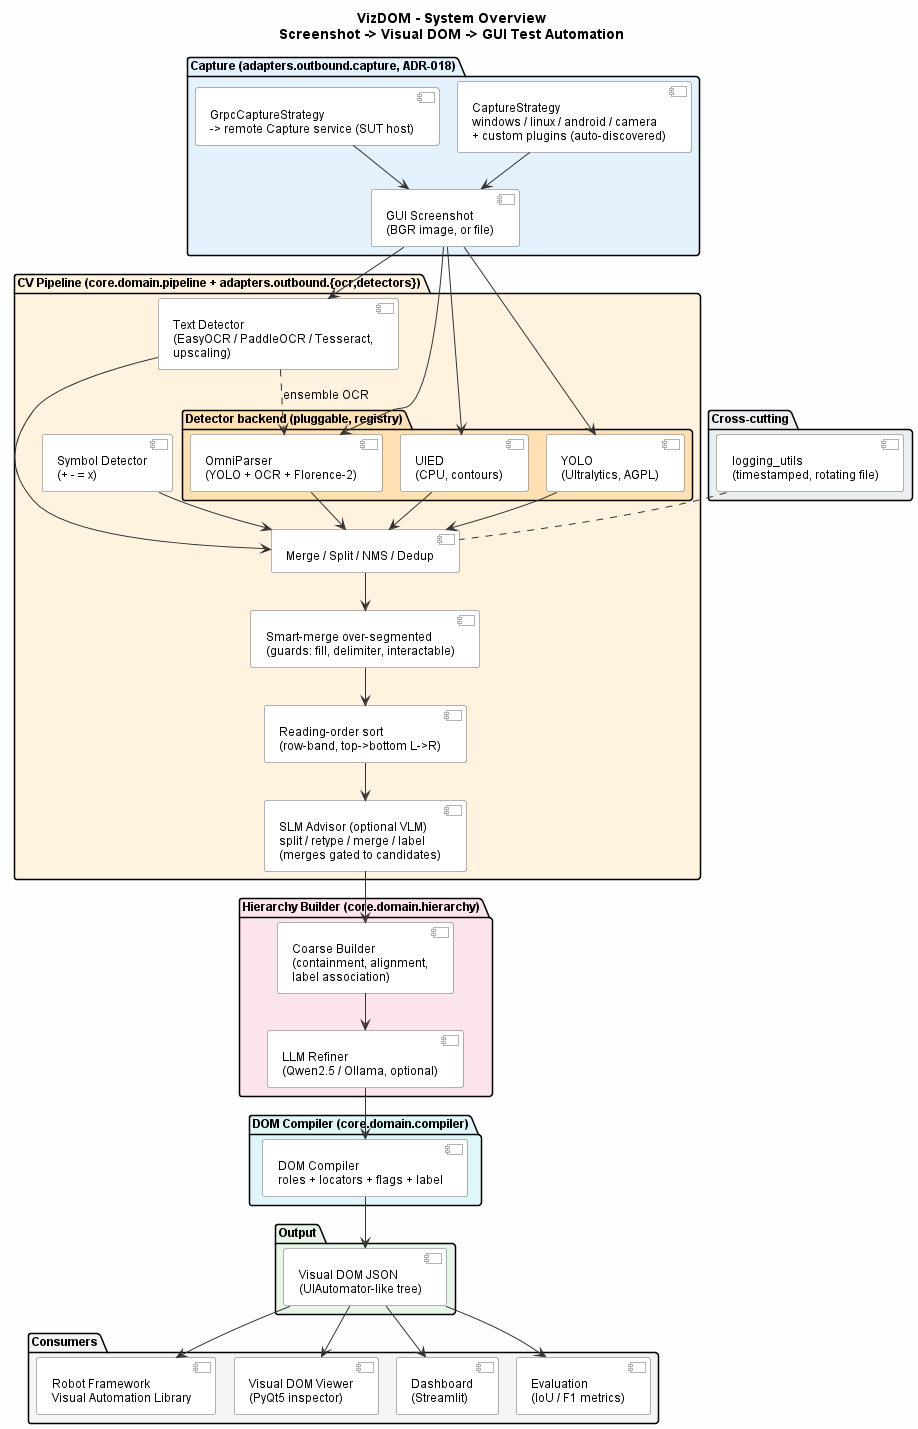
\includegraphics[width=0.62\linewidth]{System_Overview.png}
  \caption{System overview: screenshot $\rightarrow$ Visual DOM $\rightarrow$ test
  automation. Capture feeds the CV pipeline; a pluggable detector and an OCR layer
  produce elements that are merged, ordered, optionally refined by a small model,
  assembled into a hierarchy, and compiled into a DOM consumed by downstream tools.}
  \label{fig:overview}
\end{figure}

% =====================================================================
\section{Background and Related Work}
% =====================================================================

\subsection{Accessibility-based automation}
UI Automator, Windows UIA, and the web DOM give test frameworks a tree of
addressable elements \cite{uiautomator,appium}. VizDOM targets exactly the cases
where such a tree is absent or untrustworthy, and aims to \emph{synthesise} a
comparable tree from pixels.

\subsection{Image-based automation}
Sikuli and similar tools \cite{yeh2009sikuli} locate elements by template matching
on screenshots. This is robust to missing accessibility data but is
position/appearance-brittle and yields no structured hierarchy, no roles, and no
text-based locators. VizDOM instead produces a full element tree.

\subsection{The GUI element-detection problem space}
Detecting elements in a GUI is not the same task as object detection in natural
images; the study VizDOM builds on \cite{xie2020uied} identifies GUI-specific
difficulties at two levels. At the \emph{element} level: (i) \emph{large intra-class
variation} --- one class such as \code{button} or \code{input\_field} varies widely
in size, shape, colour and styling across designers and content; and (ii) \emph{high
inter-class similarity} --- different classes can look almost identical (a button
versus a spinner), separated only by a subtle cue such as a thin border or a small
glyph. At the \emph{GUI} level: (iii) a \emph{heterogeneous mix} of widgets, images
and text co-occur and abut one another; (iv) interfaces are often \emph{dense}, with
elements packed close together and separated by only a few pixels; and (v)
applications require \emph{high-precision region} detection --- a loose box that would
suffice to recognise an object in a photo is not enough to drive or assert on a
control. These properties directly motivate VizDOM's clean-up stages: the smart-merge
and reading-order steps (Section~\ref{sec:impl}) exist to cope with dense, adjacent
and over-segmented elements, and the box-convention effects seen in the evaluation
(Section~\ref{sec:eval}) are a direct consequence of the high-precision requirement.
Figure~\ref{fig:problemspace} summarises this taxonomy.

\begin{figure}[H]
  \centering
  \includegraphics[width=0.86\linewidth]{Problem_Space.png}
  \caption{The GUI element-detection problem space, at the element and GUI levels
  (after Xie et al.~\cite{xie2020uied}). These difficulties motivate VizDOM's
  clean-up stages and explain the box-convention effects in the evaluation.}
  \label{fig:problemspace}
\end{figure}

\subsection{Solution space: classical, deep, or a combination}
For \emph{non-text} elements two method families compete. \emph{Classical} computer
vision aggregates edges/contours and regions; it is training-free and interpretable
but its real-world visual features map poorly onto flat, synthetic GUI shapes and it
struggles on GUIs that embed real images. \emph{Deep} detectors regress bounding
boxes --- anchor-based families (Faster~R-CNN, YOLO) or anchor-free designs
(CenterNet); they generalise well but are sensitive to anchor definitions,
hyper-parameters and training data, and box regression can miss the precision GUIs
demand. The founding study's empirical finding \cite{xie2020uied} is that a
\emph{combination} --- classical region proposal for accurate non-text boxes plus a
deep model for classification, with a separate path for text --- outperforms either
family alone. For \emph{text}, off-the-shelf OCR (e.g.\ Tesseract) is the common tool,
but GUI text differs from document text (noisy backgrounds, proximity to widgets), so
scene-text models and GUI-specific handling are often needed.

VizDOM is an engineering realisation of this ``old-fashioned, deep, or a
combination?'' question: its pluggable detector port makes the classical baseline
(UIED), deep detectors (YOLO, OmniParser) and a hybrid selectable and directly
comparable (Section~\ref{sec:arch}), while its OCR layer and ensemble address the text
path. The evaluation (Section~\ref{sec:eval}) is exactly the like-for-like comparison
this framing calls for.

\subsection{GUI element detection and grounding}
Classical detection (UIED \cite{xie2020uied}) combines connected-component / edge
analysis with OCR to find text and non-text widgets on clean UIs. Learned
detectors --- YOLO family models \cite{ultralytics} and, more recently,
vision grounding systems such as Microsoft OmniParser \cite{omniparser2024}
(a YOLO icon detector plus a Florence-2 \cite{florence2} caption model plus OCR)
--- localise and describe interactive elements with strong generalisation. Recent
instruction-grounding models (Aria-UI \cite{ariaui2024}) and grounding benchmarks
(OSWorld-G/Jedi \cite{osworldg}) target ``given an instruction, point to the
element,'' which is complementary to VizDOM's goal of producing a
\emph{complete} tree rather than a single grounded point. VizDOM treats these
detectors as interchangeable backends rather than committing to one.

\subsection{OCR}
Text is recovered with EasyOCR \cite{easyocr} and/or Tesseract \cite{tesseract},
with upscaling for small text; VizDOM additionally uses OCR as an \emph{ensemble}
signal fed into OmniParser to recover text the detector alone misses.

\subsection{A comparative view of the landscape}
Recent GUI-understanding systems fall into two families. \emph{Parsers} answer
``what is on the screen?'' by enumerating elements (UIED, OmniParser, and VizDOM);
\emph{grounders} answer ``where is $X$?'' by returning a single location for a
natural-language instruction (Aria-UI \cite{ariaui2024}, ELAM-7B \cite{elam7b}, and
Jedi/OSWorld-G \cite{osworldg}). The two are complementary rather than
interchangeable. Table~\ref{tab:models} summarises the systems, and
Table~\ref{tab:capability} contrasts their capabilities.

\begin{table}[H]
  \centering\footnotesize
  \caption{The GUI-understanding landscape. ``n/v'' = licence not yet verified.
  Figures are as reported by each system's authors.}
  \label{tab:models}
  \begin{tabular}{@{}p{2.4cm}p{2.5cm}p{2.7cm}p{0.8cm}p{2.3cm}p{2.0cm}@{}}
    \toprule
    System & Paradigm & Output granularity & GPU & Base / size & License \\
    \midrule
    VizDOM (ours) & parser (CV + SLM) & hierarchical DOM tree & No$^\ast$ & composed pipeline & per backend \\
    UIED & classical CV & flat elements & No & --- & research \\
    OmniParser V2 & detector + caption & flat labelled boxes + interactability & Yes & YOLOv8 + Florence-2 & AGPL-3.0 / MIT \\
    Aria-UI & vision grounding & single point $[0,1000]$ & Yes & Aria MoE (3.9B act.) & n/v \\
    ELAM-7B & grounding + eval & point + PASSED/FAILED & Yes & Molmo-7B-D (Qwen2-7B) & Apache-2.0 \\
    Jedi-3B/7B & vision grounding & single point & Yes & 3B / 7B & n/v \\
    \bottomrule
  \end{tabular}\\[0.3em]
  {\footnotesize $^\ast$ CPU via the UIED backend; the OmniParser backend needs a GPU for practical speed.}
\end{table}

Two observations drive VizDOM's design. First, \emph{no system in this landscape
produces a hierarchy}: OmniParser emits a flat list of labelled boxes, and the
grounders emit a single point. Second, all of them target autonomous \emph{agents},
whose requirements (task success, autonomy) differ fundamentally from
\emph{testing}, which needs determinism, repeatability, reuse, and diagnosability.

\begin{table}[H]
  \centering\footnotesize
  \caption{Capability matrix. ``Y'' = yes; ``pt'' = point only; ``flat'' = flat list.}
  \label{tab:capability}
  \begin{tabular}{@{}p{5.2cm}ccccc@{}}
    \toprule
    Capability & Ours & OmniP. & Aria-UI & ELAM & Jedi \\
    \midrule
    Enumerates all elements & Y & Y & no & no & no \\
    Emits bounding boxes & Y & Y & pt & pt & pt \\
    Hierarchy / DOM tree & Y & flat & no & no & no \\
    Grounds from NL instruction & via DOM & no & Y & Y & Y \\
    Pass/fail evaluation built in & via RF & no & no & Y & no \\
    Reusable across many actions & Y & Y & re-infer & re-infer & re-infer \\
    Runs without GPU & Y & partly & no & no & no \\
    Target consumer & testing & agents & agents & HMI test & agents \\
    \bottomrule
  \end{tabular}
\end{table}

\subsection{Benchmarks, and why they cannot be pooled}
Table~\ref{tab:bench} lists author-reported scores. They come from \emph{different
benchmarks of different difficulty} and must not be placed in a single ranking;
doing so would be methodologically invalid. The pattern across them is nonetheless
instructive: single-step grounding on easy benchmarks looks nearly solved
(82--88\%), but on realistic benchmarks it falls to 40--54\%, and end-to-end agentic
task success sits between 15\% and 50\%. The bottleneck is therefore not grounding
accuracy but \emph{reliable, structured, repeatable execution} --- precisely the
argument for a deterministic DOM in a testing context.

\begin{table}[H]
  \centering\footnotesize
  \caption{Author-reported benchmark scores. \textbf{Different benchmarks --- not
  directly comparable}; shown to illustrate the easy-vs-realistic gap, not to rank.}
  \label{tab:bench}
  \begin{tabular}{@{}p{3.0cm}p{4.4cm}p{3.0cm}p{3.2cm}@{}}
    \toprule
    System & Benchmark & Score & Note \\
    \midrule
    ELAM-7B & AutomotiveUI-Bench-4K & 87.6\% / 78.2\% & ground / eval; automotive \\
    Aria-UI & ScreenSpot & 82.4\% & easy, single-step \\
    Jedi-7B & OSWorld-G (564) & 54.1\% & vs UI-TARS-7B 47.5\% \\
    OmniParser V2 & ScreenSpot Pro & 39.5\% & deliberately hard \\
    Aria-UI & OSWorld (agentic) & 15.15\% & end-to-end task success \\
    Jedi-7B + o3 & OSWorld (agentic) & 50.2\% & vs 23\% baseline \\
    \bottomrule
  \end{tabular}
\end{table}

\subsection{Positioning of VizDOM}
Element detection is now a commoditised layer: an industrial lab (OmniParser)
converged on the same ``CV owns geometry, a model adds semantics'' decomposition,
which both validates the instinct and removes detection as a differentiator. What
remains genuinely distinctive is: (i) \emph{hierarchy construction} --- containment,
alignment, and label association compiled into a queryable tree, which no compared
system produces; (ii) a \emph{testing orientation} --- locators, assertions, and
Robot Framework keywords; (iii) \emph{reuse economics} --- one parse serves many
locators and assertions, whereas grounders re-infer per instruction; and
(iv) \emph{explainability} --- an inspectable tree with traceable matching rules,
versus a coordinate from a black box. VizDOM therefore treats detectors as
interchangeable backends, using the strongest available detector while the
contribution sits in the layers above it.

\subsection{Benefits of a generated DOM for GUI testing}
\label{sec:dombenefits}
The automation methodologies surveyed above trade off along the same axes;
Table~\ref{tab:methods} contrasts them. Coordinate- and image-based scripts need no
platform support but break on any layout, theme, or resolution change and carry no
element semantics. \emph{Accessibility-tree} automation (Appium, Selenium,
UIAutomator) is the gold standard \emph{when a tree exists} --- but it is exactly
absent for custom-rendered Qt/OpenGL canvases, games, embedded HMIs, and any screen
observed through a camera or video stream. \emph{Per-instruction VLM grounding}
works without a tree but returns a single coordinate per natural-language
instruction: it is non-deterministic, re-infers with a large model on every action,
and produces no reusable structure.

A generated Visual DOM occupies the gap: it \emph{synthesises} an
accessibility-tree-like artifact from pixels alone, so tree-style testing becomes
available on UIs that have no tree. Concretely this buys four things a test suite
depends on. (i) \textbf{Universality} --- it works wherever there are pixels
(custom-rendered, embedded, remote, camera), the very cases where
instrumentation-based tools cannot run. (ii) \textbf{Semantic, resilient locators}
--- roles, text, labels and spatial relations replace brittle pixel coordinates, so
a test survives repositioning and restyling. (iii) \textbf{A reusable, inspectable
artifact} --- one parse yields a queryable JSON tree that serves many locators and
assertions and can be diffed, logged and audited, unlike a per-step grounding call.
(iv) \textbf{Lower, bounded cost} --- perception runs once per screen (and can use a
CPU backend) instead of invoking a large model per action. The price is that
perception is approximate: detection and captioning can miss or mislabel elements
(the per-type recall of Table~\ref{tab:pertype}), so the DOM is a best-effort
reconstruction rather than ground truth --- which is why VizDOM keeps the detector
pluggable and reports recall per element type rather than a single headline score.

\begin{table}[H]
  \centering\footnotesize
  \caption{GUI-test methodologies against the requirements a test suite cares about.
  ``Part.'' = partial.}
  \label{tab:methods}
  \begin{tabular}{@{}p{3.0cm}p{1.7cm}p{1.6cm}p{1.6cm}p{1.6cm}p{1.5cm}@{}}
    \toprule
    Methodology & Works w/o a11y tree & Custom / camera & Structured tree & Resilient locators & Reusable artifact \\
    \midrule
    Coordinate / record--replay & Yes & Yes & No & No & Part. \\
    Image / template match & Yes & Yes & No & No & Part. \\
    Accessibility tree (Appium/UIAutomator) & No & No & Yes & Yes & Yes \\
    VLM grounding (per instruction) & Yes & Yes & No & Part. & No \\
    \textbf{VizDOM (generated DOM)} & Yes & Yes & Yes & Yes & Yes \\
    \bottomrule
  \end{tabular}
\end{table}

% =====================================================================
\section{System Architecture}
\label{sec:arch}
% =====================================================================

\subsection{Hexagonal ports and adapters}
VizDOM is structured as a hexagonal architecture (Figure~\ref{fig:arch}). A pure,
local domain core (pipeline orchestration, reading-order and merge logic, coarse
hierarchy building, DOM compilation) depends only on abstract \emph{ports};
concrete adapters are selected at run time. There are five driven ports:
\begin{itemize}[leftmargin=1.4em]
  \item \textbf{DetectorPort} --- find elements (UIED, YOLO, OmniParser, or a
        remote detector);
  \item \textbf{OcrPort} --- recover text;
  \item \textbf{RefinerPort} --- optional small-model review;
  \item \textbf{CapturePort} --- read the screen; and
  \item \textbf{ActuatorPort} --- drive input.
\end{itemize}
Driving adapters (the CLI, the PyQt5 Viewer, a Streamlit dashboard, and the Robot
Framework library) enter the core through pipeline orchestration.

\begin{figure}[H]
  \centering
  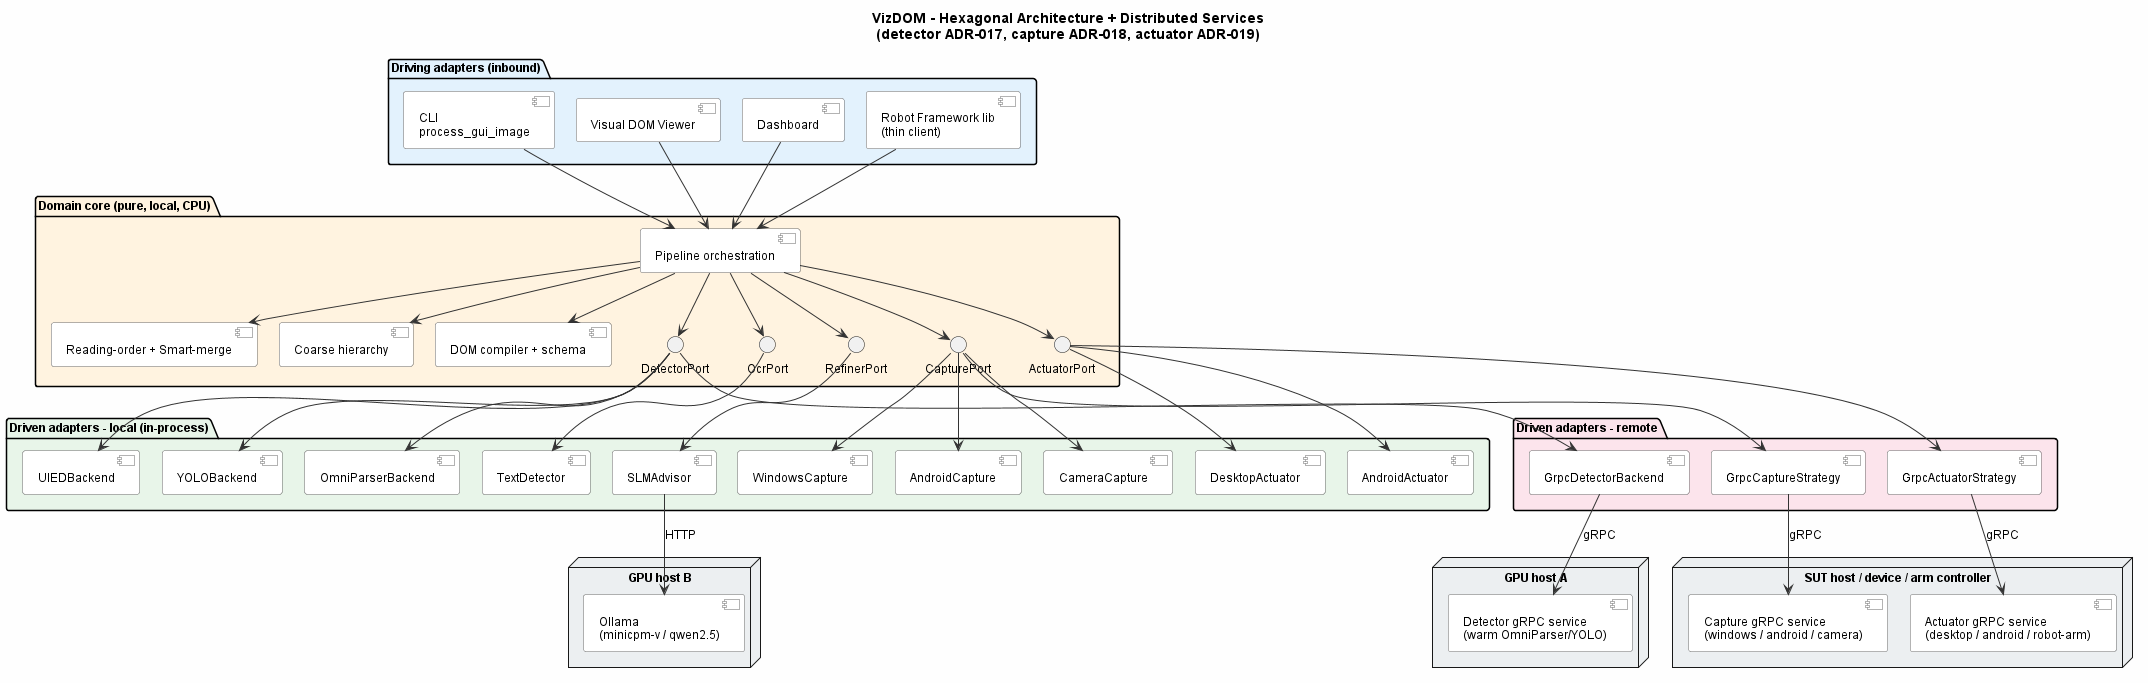
\includegraphics[width=\linewidth]{Architecture.png}
  \caption{Hexagonal architecture with distributed services. Capture, detection,
  and actuation are driven ports; each has in-process adapters and a remote gRPC
  adapter, so services can run on the device under test, a GPU host, and a
  robot-arm controller respectively.}
  \label{fig:arch}
\end{figure}

\subsection{Pluggable strategies and auto-discovery}
Each of the capture, detector, and actuator ports uses the same pattern: a strategy
base class, a registry, and \emph{auto-discovery} of user plugins dropped into a
conventional folder (e.g. \code{plugins/capture/}, \code{plugins/actuator/}). A user
adds a new capture source or a new way to actuate the system --- a camera, a
capture card, or a robot arm --- by writing one file that subclasses the strategy
base; the registry loads it on the next run and it is selected by name from
configuration. This makes the system extensible without modifying the core.

\subsection{Distributed deployment via gRPC}
Because capture runs where the application under test is, detection benefits from a
GPU, and actuation happens at the device or a physical controller, each port also
has a remote adapter backed by a gRPC service \cite{grpc}. A warm-model
\emph{detector} service loads a heavy model once and serves many lightweight
clients; a \emph{capture} service serves screenshots from the device; an
\emph{actuator} service performs input on the device or drives a robot arm.
Crucially, gRPC is a transport, not a requirement: a local desktop run uses the
in-process adapter with no server, while the \code{grpc} strategy is selected only
when the port lives on another machine. A representative distributed configuration
is: \emph{capture on the device $\rightarrow$ detect on a GPU host $\rightarrow$
actuate on the SUT / robot-arm controller $\rightarrow$ orchestrate on the client}.

\subsection{Coordinate contract for actuation}
Detection yields coordinates in image pixels, but where an action lands depends on
the actuator's own space. VizDOM's actuator contract therefore uses
\emph{normalized} coordinates in $[0,1]$ plus the source image size; each strategy
maps them to its device space: a desktop multiplies by screen resolution, an
Android device by its input resolution, and a robot-arm plugin applies a
calibration homography from image pixels to physical servo coordinates. This keeps
the orchestrator and the network protocol independent of any device's resolution.

\subsection{Architectural decisions and trade-offs}
\paragraph{Ports and adapters over a layered monolith.} The domain core depends only
on abstract ports, not on concrete detectors, capture sources, or actuators. This
hexagonal style is chosen for testability (the core runs with no I/O) and
substitutability (backends swap without touching business logic); the accepted cost
is the indirection of an interface and a registry per port, judged worthwhile
because substitutability is the project's primary quality goal.

\paragraph{Optional service extraction, not always-on microservices.} VizDOM is a
\emph{modular monolith} that can extract individual ports into services on demand,
rather than a system pre-decomposed into always-running microservices. Distribution
is driven by \emph{physical locality and resource}, not by fashion: capture must run
where the app-under-test is, detection benefits from a GPU, and actuation happens at
the device. A single in-process run remains the default, avoiding the operational
tax (deployment, service discovery, partial-failure handling) that an
always-distributed design would impose on the common case.

\paragraph{gRPC over REST or a message broker.} Remote ports use gRPC because its
typed protobuf contracts fit a stable cross-machine interface, its binary framing
carries image bytes without base64 inflation, and its unary request/response maps
directly onto ``grab a frame'' / ``run detection'' / ``perform a tap''. REST+JSON
would inflate image payloads and lose the typed contract; a message broker would add
infrastructure the no-container constraint rules out and impose asynchronous
semantics on operations that are naturally synchronous.

\paragraph{In-process by default.} The gRPC path is selected only when a port lives
on another machine; a local desktop run pays no network, serialisation, or
server-lifecycle cost. This keeps the simple case simple and the distributed case
possible with the \emph{same} code, and is the concrete mechanism behind the
deployability quality goal.

% =====================================================================
\section{Implementation}
\label{sec:impl}
% =====================================================================

\subsection{The CV pipeline}
The core transformation is \code{VisualDOMPipeline.process()}
(Figure~\ref{fig:pipeline}). Its stages are:
\begin{enumerate}[leftmargin=1.6em]
  \item \textbf{Acquire and prepare.} A screenshot is obtained (via a capture
        strategy or a file), optionally rectified in ``camera mode,'' and a
        resolution-aware scale factor is computed.
  \item \textbf{Text detection.} An OCR engine (EasyOCR/PaddleOCR/Tesseract) with
        upscaling produces text elements.
  \item \textbf{Element detection.} A pluggable detector backend runs: UIED
        (CPU contour analysis), YOLO, OmniParser (YOLO icon detection + Florence-2
        captions + OCR), or a hybrid, producing detections that are normalised to a
        common \code{UIElement} form.
  \item \textbf{Merge / split / de-duplicate.} Text and elements are merged by
        containment/IoU, split by text positions, and reduced with
        cross-type and per-type non-maximum suppression.
  \item \textbf{Smart-merge of over-segmentation.} Fragment boxes that form one
        logical element (a multi-line button, a split text line) are merged under
        guards --- a fill-ratio threshold, a delimiter check, and an
        ``at most one interactable member'' rule --- to avoid fusing distinct
        controls.
  \item \textbf{Reading-order sort.} Elements are ordered top-to-bottom,
        left-to-right using a row-band heuristic.
  \item \textbf{Optional SLM/VLM review.} A small model served by Ollama may
        split, re-type, merge, and \emph{label} suspicious elements; merges are
        gated to geometrically pre-approved candidates so the model cannot fuse
        unrelated controls.
  \item \textbf{Hierarchy and output.} A coarse builder infers containment,
        alignment groups, and label associations; the DOM compiler emits roles,
        interaction flags, multiple locators, and human-readable labels.
\end{enumerate}

\begin{figure}[H]
  \centering
  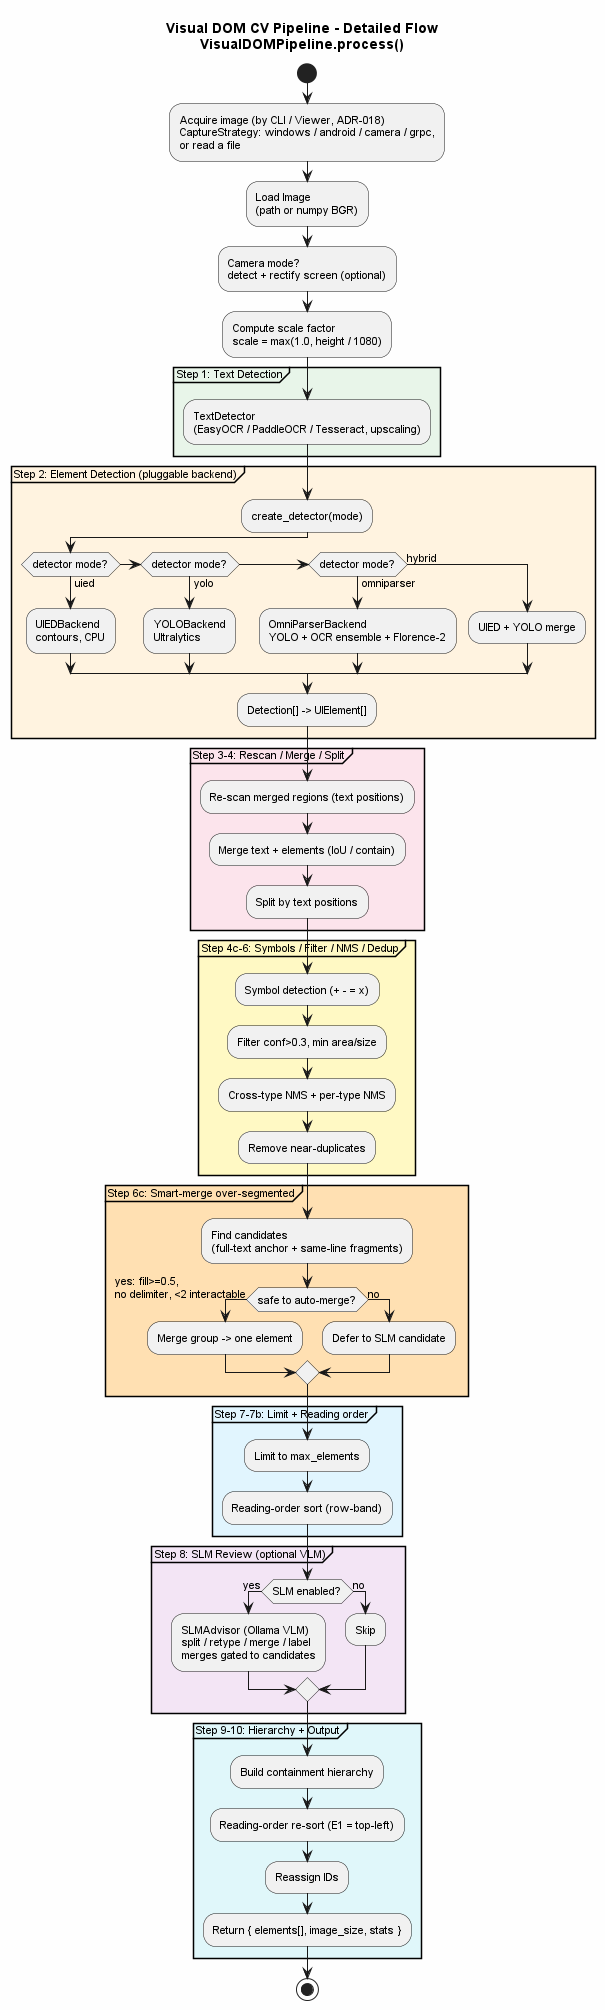
\includegraphics[height=0.86\textheight,width=\linewidth,keepaspectratio]{CV_Pipeline_Detail.png}
  \caption{Detailed control flow of \code{VisualDOMPipeline.process()}: acquire,
  OCR, pluggable detection, clean-up, smart-merge, reading-order, optional
  small-model review, and hierarchy/DOM output.}
  \label{fig:pipeline}
\end{figure}

\subsection{Pipeline design decisions}
The pipeline's shape follows from a small number of decisions, each a response to an
observed failure mode:
\begin{itemize}[leftmargin=1.4em]
  \item \textbf{Pluggable detector, not a single model.} Detection quality varies by
        UI style and by available hardware; a stable \code{detect(image)} interface
        lets a CPU baseline (UIED) and a GPU grounding model (OmniParser) coexist and
        be compared, and lets an AGPL detector be replaced by a permissive one
        without touching the pipeline. Trade-off: two or more code paths to maintain.
  \item \textbf{OCR ensemble.} A learned detector localises interactive elements well
        but misses fine text; feeding an upscaling OCR pass into the detector
        recovers missed words (gap-fill de-duplication). Trade-off: a second OCR pass
        costs time, so it is optional.
  \item \textbf{Guarded rule-based smart-merge \emph{before} the model.} OmniParser
        tends to over-segment (a multi-line button becomes several boxes). Merging
        fragments by fill-ratio, delimiter, and an ``at most one interactable
        member'' guard is deterministic, cheap, and explainable, and avoids fusing
        distinct controls. Trade-off: hand-tuned thresholds.
  \item \textbf{Small-model refinement, gated.} A small LM/VLM reviews only
        suspicious elements (split / re-type / merge / label), and its merges are
        restricted to geometrically pre-approved candidates, so a probabilistic model
        can never fuse unrelated controls. Trade-off: a model dependency --- hence
        optional, degrading gracefully when absent.
  \item \textbf{Geometry from CV, semantics from the model.} The pipeline never lets
        the language model emit coordinates; it owns only labels and types. This
        division of labour --- validated independently by OmniParser's design ---
        keeps spatial accuracy deterministic while using the model where it is strong.
\end{itemize}

\subsection{Pluggable detector backends}
Detectors implement a common \code{DetectorBackend} interface
(\code{detect(image)} $\rightarrow$ \code{List[Detection]}, \code{is\_available()}) and are built by a
registry factory. UIED is a dependency-free CPU baseline; YOLO and OmniParser are
learned backends; a gRPC backend forwards to a remote warm-model service. In
practice OmniParser separates closely packed controls (e.g.\ calculator buttons)
better than UIED but tends to over-segment, which motivates the rule-based
smart-merge and the guarded small-model refinement above.

\subsection{From detections to a DOM}
The coarse hierarchy builder associates labels with controls (e.g.\ a field and its
caption), groups aligned elements, and nests by containment. The DOM compiler then
produces a UI-Automator-like JSON tree: each node carries an id, bounds, center,
role, visual type, interaction flags (clickable/editable/scrollable), an optional
text and label, and multiple \emph{locators} (by id, text, hint, role, and spatial
relations).

\subsection{Robot Framework Visual Automation Library}
The second deliverable is a Robot Framework library \cite{robotframework} that acts
as a thin orchestrator over the capture and actuator ports. Representative keywords:
\begin{itemize}[leftmargin=1.4em]
  \item \emph{Capture / analysis}: \code{Capture Screen}, \code{Dump Visual DOM},
        \code{Load Visual DOM};
  \item \emph{Queries}: \code{Get Visual Element}, \code{Get Element Property},
        \code{Get Element Text}, \code{Get Element Label}, \code{Get Element Center};
  \item \emph{Actions}: \code{Click Visual}, \code{Type Text Visual},
        \code{Press Key}, \code{Scroll Visual}, \code{Drag And Drop Visual};
  \item \emph{Assertions / waits}: \code{Visual Should Exist},
        \code{Visual Should Not Exist}, \code{Wait Until Visual Appears},
        \code{Wait Until Visual Disappears}.
\end{itemize}
Locators support \code{id=}, \code{text=}, \code{hint=}, \code{role=}, and spatial
relations (\code{within=}, \code{right\_of=}, \code{below=}, \dots). Actions resolve
a locator to an element, convert its center to normalized coordinates, and delegate
to the actuator, so the same test runs locally, over gRPC, or against a robot arm
without change. Figure~\ref{fig:seq} shows the end-to-end interaction for a single
screenshot-to-DOM cycle.

\begin{figure}[H]
  \centering
  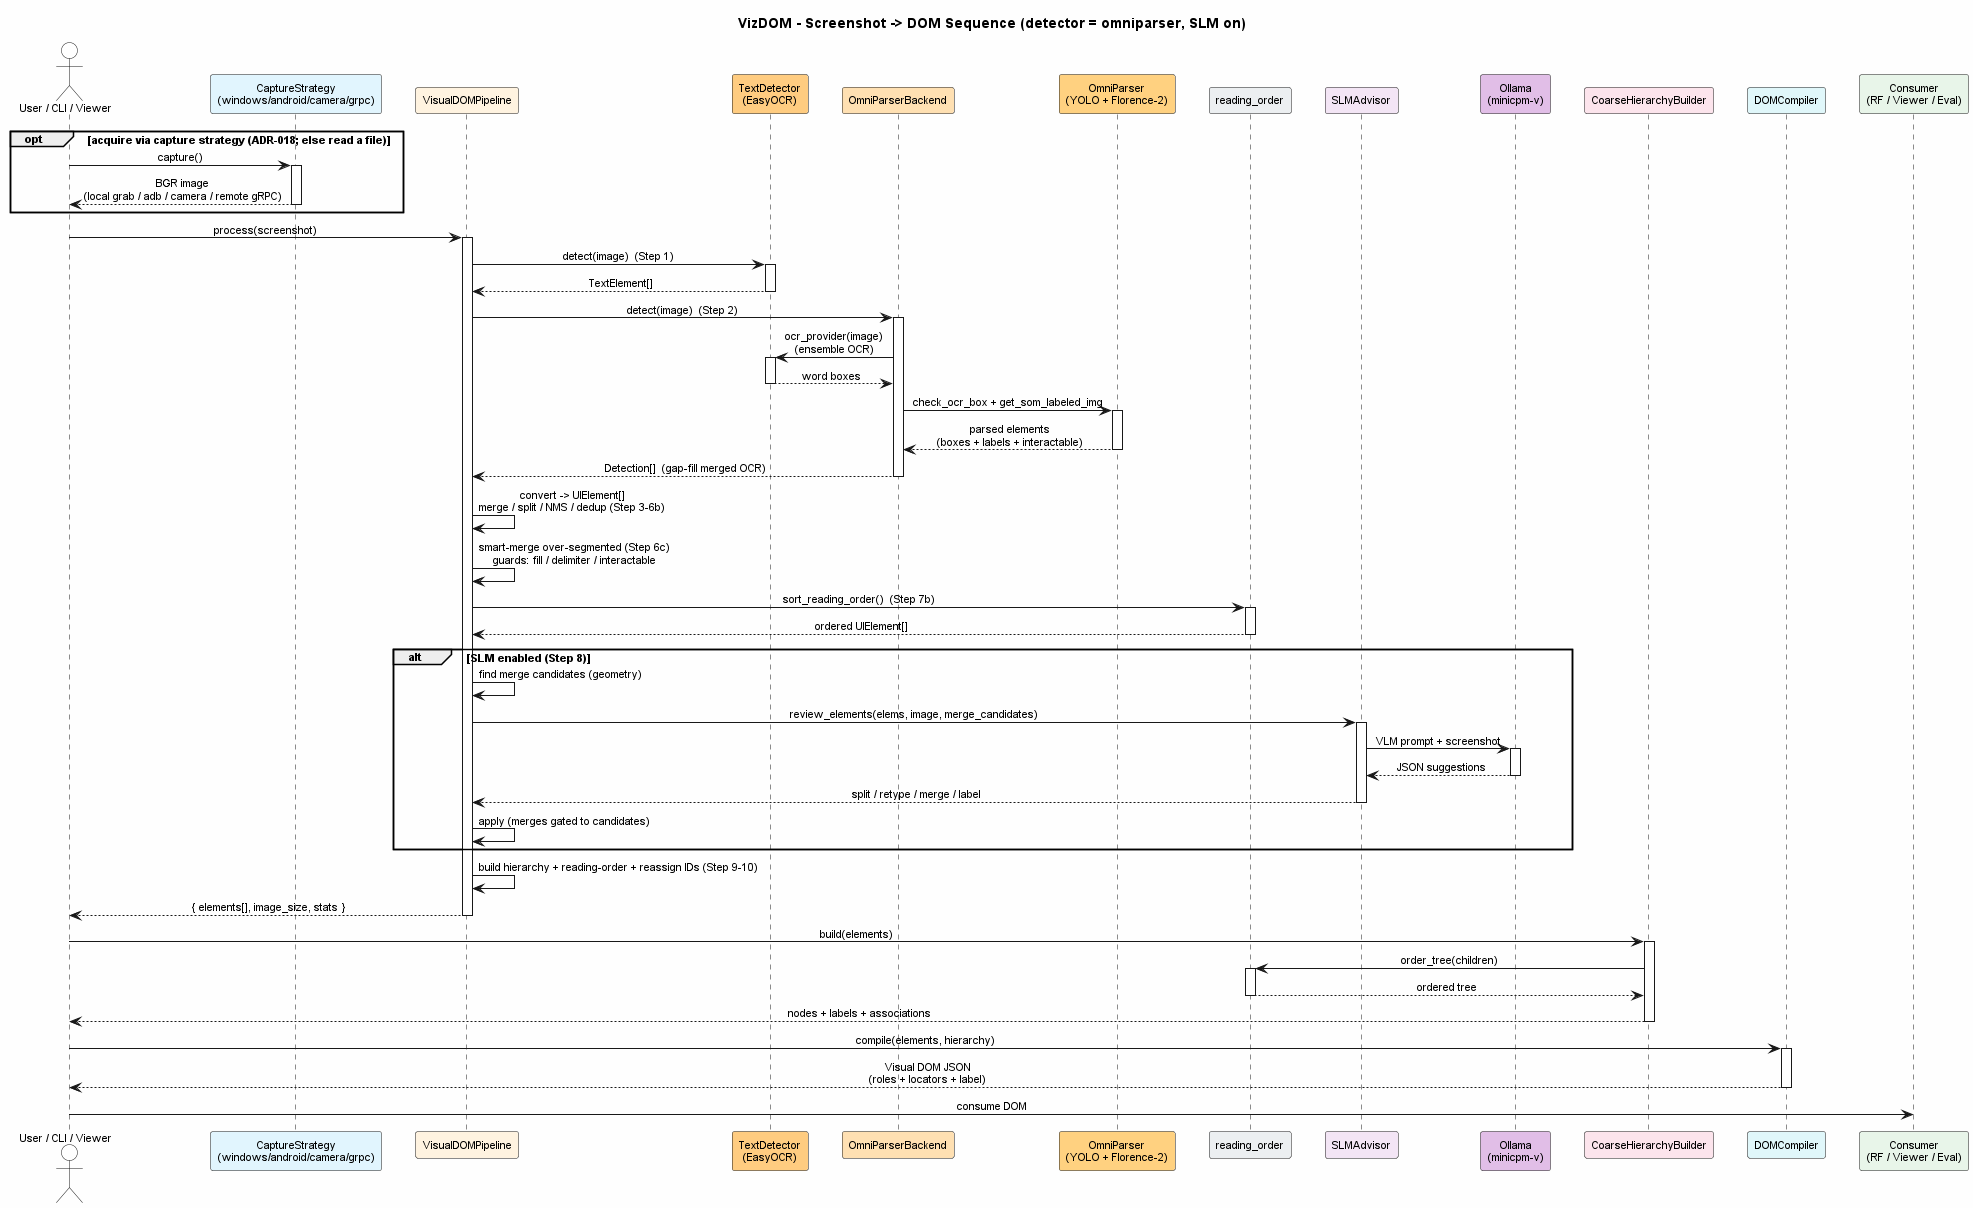
\includegraphics[width=\linewidth]{Sequence_Diagram.png}
  \caption{Sequence of a screenshot-to-DOM cycle (detector = OmniParser, SLM
  enabled): optional capture, OCR, detection with OCR ensemble, clean-up,
  reading-order, optional small-model review, hierarchy building, and DOM
  compilation for the consumer.}
  \label{fig:seq}
\end{figure}

\subsection{Engineering environment}
The system runs on Python~3.9 with a CUDA-enabled PyTorch build; environments are
managed with \code{uv}. Development is behind a corporate proxy that blocks public
code hosts, which shaped several decisions: external model code is vendored and
pinned by a setup script rather than fetched as a submodule, and the documentation
site renders its UML diagrams fully offline from a local renderer. Supporting tools
include a PyQt5 Visual DOM Viewer (capture, inspect, export), a Streamlit
dashboard, and an annotation tool.

% =====================================================================
\section{Evaluation}
\label{sec:eval}
% =====================================================================

\subsection{Methodology}
Quality is assessed along four axes with an evaluation harness:
\begin{itemize}[leftmargin=1.4em]
  \item \textbf{Element detection}: precision, recall, F1, and mean IoU against
        annotated ground-truth boxes;
  \item \textbf{OCR}: character accuracy and character-/word-error rates (CER/WER);
  \item \textbf{Hierarchy}: correctness of containment/label association; and
  \item \textbf{Locator quality}: uniqueness and stability of generated locators.
\end{itemize}
The benchmark is a \textbf{synthetic UI dataset} (programmatically generated
screenshots at $1920\times1080$ with exact ground truth --- element bounds,
\code{visual\_type}, text, and containment --- in the same schema the pipeline
emits), split into 167 training and \textbf{44 test} images. Predictions are the
pipeline's elements for each test image; matching is greedy by IoU at a
threshold of 0.5. Because the ground truth is a flat element list with parent
references (not a nested tree) and carries no locators, the element-detection and
OCR axes are reported here; hierarchy and locator axes require tree/locator-bearing
ground truth and are left to future annotated data. All figures are computed by the
project's own evaluation harness (\code{visual\_dom.evaluation}).

\subsection{Functional verification}
The end-to-end system and its distributed services were verified functionally:
\begin{itemize}[leftmargin=1.4em]
  \item the full pipeline processes a reference UI screenshot and emits a
        well-formed DOM (dozens of elements with roles, locators, and labels);
  \item the \textbf{detector} gRPC service loads a warm model once and returns
        detections to a remote client;
  \item the \textbf{capture} gRPC service returns a pixel-identical screenshot to a
        remote client; and
  \item the \textbf{actuator} gRPC service reproduces normalized actions exactly,
        mapping them to device coordinates server-side (verified end-to-end with a
        recording actuator and a robot-arm homography stub).
\end{itemize}

\subsection{Quantitative results on the synthetic benchmark}
Table~\ref{tab:results} reports overall (pooled) element-detection and OCR metrics
on the 44-image synthetic test set; Table~\ref{tab:pertype} breaks recall down by
element type --- far more informative for a testing use case --- under two lenses:
strict overlap (IoU $\geq 0.5$) and \emph{click-targetability} (``center-hit'': does
a predicted box contain the element's centre, so a test could click it?).

\begin{table}[H]
  \centering
  \caption{Overall element detection and OCR on the synthetic test set (44 images,
  IoU threshold 0.5, greedy matching, pooled over all elements). Higher is better.}
  \label{tab:results}
  \begin{tabular}{lccccc}
    \toprule
    Detector & Precision & Recall & F1 & mIoU & Char.\ acc. \\
    \midrule
    UIED (CPU)   & 0.39 & \textbf{0.71} & 0.51 & 0.68 & 0.92 \\
    OmniParser   & \textbf{0.56} & 0.59 & \textbf{0.58} & \textbf{0.67} & \textbf{0.95} \\
    YOLO         & \multicolumn{5}{c}{\emph{not evaluated --- no trained weights for these UI classes}} \\
    \bottomrule
  \end{tabular}
\end{table}

\begin{table}[H]
  \centering
  \caption{Recall by ground-truth element type under two lenses: strict overlap
  (IoU$\geq$0.5) and click-targetability (a predicted box contains the element's
  centre). ``n'' = count in the 44-image test set. Actionable = button + input +
  checkbox + icon.}
  \label{tab:pertype}
  \begin{tabular}{lc cc cc}
    \toprule
    & & \multicolumn{2}{c}{UIED} & \multicolumn{2}{c}{OmniParser} \\
    \cmidrule(lr){3-4}\cmidrule(lr){5-6}
    GT type & n & IoU$\geq$0.5 & center-hit & IoU$\geq$0.5 & center-hit \\
    \midrule
    button       & 183  & 0.82 & 0.96 & \textbf{1.00} & \textbf{1.00} \\
    input\_field & 135  & 0.95 & 0.99 & \textbf{0.99} & 0.99 \\
    checkbox     & 76   & \textbf{0.68} & 0.82 & 0.20 & \textbf{0.87} \\
    icon         & 36   & 0.08 & 0.28 & \textbf{0.67} & \textbf{1.00} \\
    text         & 1074 & \textbf{0.79} & \textbf{0.99} & 0.59 & 0.98 \\
    block        & 51   & 0.55 & 0.63 & 0.37 & 0.43 \\
    divider      & 145  & 0.00 & 0.10 & 0.00 & 0.21 \\
    \midrule
    actionable (pooled) & 430 & 0.77 & 0.89 & \textbf{0.83} & \textbf{0.97} \\
    \bottomrule
  \end{tabular}
\end{table}

In aggregate the two backends are close (F1 0.51 vs.\ 0.58), but the per-type
breakdown shows they lead on different element kinds. \textbf{OmniParser is stronger
on the actionable controls a test drives}: it localises \emph{buttons} perfectly
(recall 1.00), \emph{input fields} at 0.99, and \emph{icons} at 0.67 (vs.\ UIED's
0.08), with tight boxes (mIoU 0.68) --- corroborating manual inspection that its
bounding is more accurate. \textbf{UIED leads on checkboxes} (IoU 0.68 vs.\ 0.20)
and \emph{text} recall (0.79 vs.\ 0.59). By click-targetability both are strong, and
OmniParser is essentially perfect on the actionable set (0.97 pooled; button/icon
1.00, input 0.99) versus UIED's 0.89. OmniParser's low checkbox IoU (0.20) with a
high center-hit (0.87) is the familiar box-convention effect --- it boxes the check
glyph rather than the padded control --- so the elements are clickable even when the
strict overlap is low.

Two points close the loop with the qualitative observation. First, the earlier
weakness in \emph{classification} (OmniParser labelling everything \code{text}/
\code{icon}) has been addressed: the backend now infers \code{button} /
\code{input\_field} / \code{checkbox} / \code{icon} from interactivity and
resolution-aware geometry, so its DOM is directly usable by the test layer. Second,
for a GUI-testing use case --- where an element mainly needs to be reliably
\emph{clickable} --- OmniParser is the stronger default on this benchmark, while
UIED remains the GPU-free baseline and the better choice where text or checkbox
recall dominates. Caveats: this is a \emph{synthetic, clean} set (absolute scores
will differ on real UIs); the OCR ensemble produced no measurable change here
(OmniParser's own OCR already captured the text); and the SLM-refinement variant was
not benchmarked (it needs a running Ollama service).

\subsection{Improving OmniParser element-type classification}
Evaluation and manual inspection surfaced a limitation orthogonal to box quality:
although OmniParser's \emph{boxes} are accurate, the integration originally mapped
every detection to only \code{text} or \code{icon}, so the DOM carried no
\code{button} / \code{input\_field} / \code{checkbox} roles --- type-classification
accuracy on actionable controls was \textbf{0\%} by construction, and role-based
test logic could not use the OmniParser DOM.

The improved mapping (\code{\_infer\_visual\_type}) combines three signals. First,
\emph{geometry}: a wide entry-height box is an input field, and a small square box a
control glyph. Second, \emph{width/aspect} separates buttons from icons --- buttons
are markedly wider (measured median width $\approx 2\times$ that of icons), so a
wide labelled box is a button and a small near-square one an icon. Third, the
OmniParser \emph{caption} disambiguates checkboxes from icons (both small squares):
captions naming ``check'', ``toggle'', ``radio'' or ``switch'' mark a checkbox.
Separately, the pipeline now auto-resolves OmniParser's model paths, since a missing
path had silently degraded a run to OCR-only.

Table~\ref{tab:typeacc} reports the effect in the two measured stages it took to
get there. The original mapping scored actionable type-accuracy of only 0.09 ---
correct solely on icons, which it obtained trivially by labelling \emph{everything}
\code{icon} (hence its inability to identify anything else). A \emph{first fix} added
the interactivity- and geometry-based role inference (input-height and width/aspect),
which recovered buttons (0.91) and input fields (0.99) and lifted actionable accuracy
to 0.73 --- but it \emph{regressed} icons: the geometry rule now reclassified small
square glyphs as buttons or checkboxes, dropping icon accuracy from its trivial 1.00
to 0.00, and checkboxes stayed near-zero (0.12) because they are geometrically
indistinguishable from icons. Adding OmniParser's \emph{caption} to disambiguate
checkboxes, and re-tuning the width/aspect boundary between buttons and icons,
produced the current mapping: icons recover to 0.89, checkboxes to 0.55, buttons
hold at 0.89, and actionable accuracy reaches \textbf{0.87}. OmniParser's DOM is now
directly usable by the test layer across all interactive roles.

\begin{table}[H]
  \centering
  \caption{Element-type classification accuracy on matched actionable controls,
  across the two improvement stages (OmniParser, synthetic test set):
  \emph{before} (text/icon only), \emph{first fix} (interactivity + geometry), and
  \emph{now} (+ caption disambiguation and re-tuned width/aspect). Localisation
  (Table~\ref{tab:pertype}) is unaffected --- this measures \emph{type} only.
  $^\dagger$The original mapping labelled all non-text as \code{icon}, so icons were
  correct trivially while every other role scored 0.}
  \label{tab:typeacc}
  \begin{tabular}{lccc}
    \toprule
    GT type & Before & First fix & Now \\
    \midrule
    button       & 0.00 & 0.91 & 0.89 \\
    input\_field & 0.00 & 0.99 & 0.99 \\
    checkbox     & 0.00 & 0.12 & 0.55 \\
    icon         & 1.00$^\dagger$ & 0.00 & \textbf{0.89} \\
    \midrule
    actionable   & 0.09 & 0.73 & \textbf{0.87} \\
    \bottomrule
  \end{tabular}
\end{table}

Checkboxes remain the weakest role (0.55): they are recovered only when OmniParser's
caption is distinctive (``Checkmark'', ``Toggle''), and many carry a generic caption
or their visible label instead. Using the adjacent text label or richer caption
semantics to identify checkboxes is left as future work.

\subsection{Efficiency considerations}
Efficiency is analysed along three axes. Wall-clock figures await the like-for-like
benchmark (Table~\ref{tab:results}), so the discussion here is structural and relies
on published model characteristics rather than unmeasured timings.

\paragraph{Hardware footprint.} The grounding models are large and GPU-bound ---
Aria-UI activates 3.9B parameters, and ELAM-7B and Jedi-7B are 7B-class --- whereas
VizDOM's UIED backend is CPU-only. A CPU path is a genuine differentiator for test
rigs and embedded targets without a GPU; the accurate-but-heavy OmniParser backend
is offered for hosts that have one.

\paragraph{Reuse economics.} A parser amortises cost: one DOM parse serves many
locator lookups and assertions ($O(1)$ model work followed by $n$ cheap tree
queries), whereas a grounder re-infers per instruction ($n$ model invocations). In a
regression suite of thousands of steps this asymptotic difference is the distinction
between a practical and an impractical tool --- a decisive efficiency argument for
the DOM abstraction in testing, independent of any single latency number.

\paragraph{Warm-model services and offload.} The detector service loads its model
once and serves subsequent requests with inference only, and one GPU host can serve a
fleet of light CPU clients. Placing capture at the device, inference on the GPU host,
and orchestration on the client keeps each node doing what it is suited to and avoids
shipping a heavy model to every machine. The planned benchmark will report
CPU-versus-GPU latency and detector throughput per the methodology above.

% =====================================================================
\section{Discussion and Limitations}
% =====================================================================
\begin{itemize}[leftmargin=1.4em]
  \item \textbf{Real-world robustness.} Detection and symbol recognition are strong
        on clean and synthetic UIs but weaker on gradient-heavy, themed
        applications; reducing over-segmentation is ongoing.
  \item \textbf{Quantitative evaluation.} Results are reported on a synthetic
        benchmark (Section~\ref{sec:eval}); a larger, \emph{real-world} labelled set
        is still needed to confirm the numbers transfer beyond clean UIs, and to
        exercise the hierarchy and locator axes the current ground truth cannot.
  \item \textbf{Calibration for physical actuation.} The robot-arm case requires a
        per-setup image-to-physical calibration; the architecture isolates this to
        the plugin, but it remains real work, and physical actuation carries safety
        obligations (work-area limits, e-stop) that a plugin must enforce.
  \item \textbf{Security of extensibility.} Plugin auto-discovery imports user code
        and gRPC channels are currently unauthenticated; both are acceptable for
        trusted/LAN use and are flagged for hardening (entry-point discovery, TLS).
\end{itemize}

% =====================================================================
\section{Conclusion and Future Work}
% =====================================================================
VizDOM demonstrates that a usable, UI-Automator-like DOM can be reconstructed from a
screenshot by composing classical computer vision, a modern vision grounding model,
and a small-model refinement stage, and that the resulting engine can be deployed
flexibly through a hexagonal, service-oriented architecture. The system already
delivers value to a real test framework and supports deployments as unconventional
as camera capture with robot-arm actuation. Future work includes: completing the
quantitative benchmark on a larger labelled dataset; reducing over-segmentation on
themed real-world UIs; evaluating instruction-grounding models (Aria-UI, ELAM-7B,
Jedi) as replacements or complements for the small-model refinement step; and
hardening the services with authentication/TLS and setuptools entry-point plugin
discovery.

\bibliographystyle{plain}
\bibliography{references}

\end{document}
